\subsection{Dataset}
	We crawled and extracted our data from YouTube for one month (Oct - Nov, 2015). The crawling strategy is akin to bread-first search. First we initialize the crawler with several random "seed" videos, which mostly are in the \textit{Movie} and \textit{Music} category, and recursively explore all other related videos recommended by YouTube recommendation systems. For each video, we extract all of its metadata such as title, uploader and his number of subscriptions, description, upload date, number of views/likes/dislikes, video length, and a number of other attributes, as well as a list of around 30 videos YouTube recommends as being similar. 

	\subsubsection{Data Statistics}
		Although the crawler was suspended twice due to technical issues and upgrades, we have gathered a sizeable amount of data, with tremendous variation in the observed values:
		
		\begin{itemize}
			\item Number of videos crawled: 1,432,213
			\item Number of uploaders: 628,072
			\item Number of "bag of word" features (extracted from the titles): 2,447,603 entries
			\item Video length: $[1 \ldots 107,373]$ (seconds)
			\item Range of number of day passed since uploaded: $[1 \ldots 3423]$ (days)
			\item Range of number of views: $[7 \ldots 2,104,518,656]$.
			\item Range of number of likes: $[1 \ldots 8,639,650]$.
			\item Range of number of dislikes: $[1 \ldots 4,184,769]$.
		\end{itemize}

		We plot in Figure \ref{fig:histograms} different histograms reflecting characteristics of our data. In the red-colorer histogram, we look for the distributions of videos and their view counts. Interestingly, the distribution is in the shape of Gaussians, instead of following the Power Law distribution as frequently observed in social networks. We guess this observation is due to the way we sampled the data, by following the recommended links. It is intuitive since videos with high view counts are usually recommended together. The Gaussian distribution also encourages us to perform some standardisation on the data, such as subtracting the label to the mean of the Gaussian and predict the left amount. 
		

		\begin{figure}[!h]
			\begin{center}
				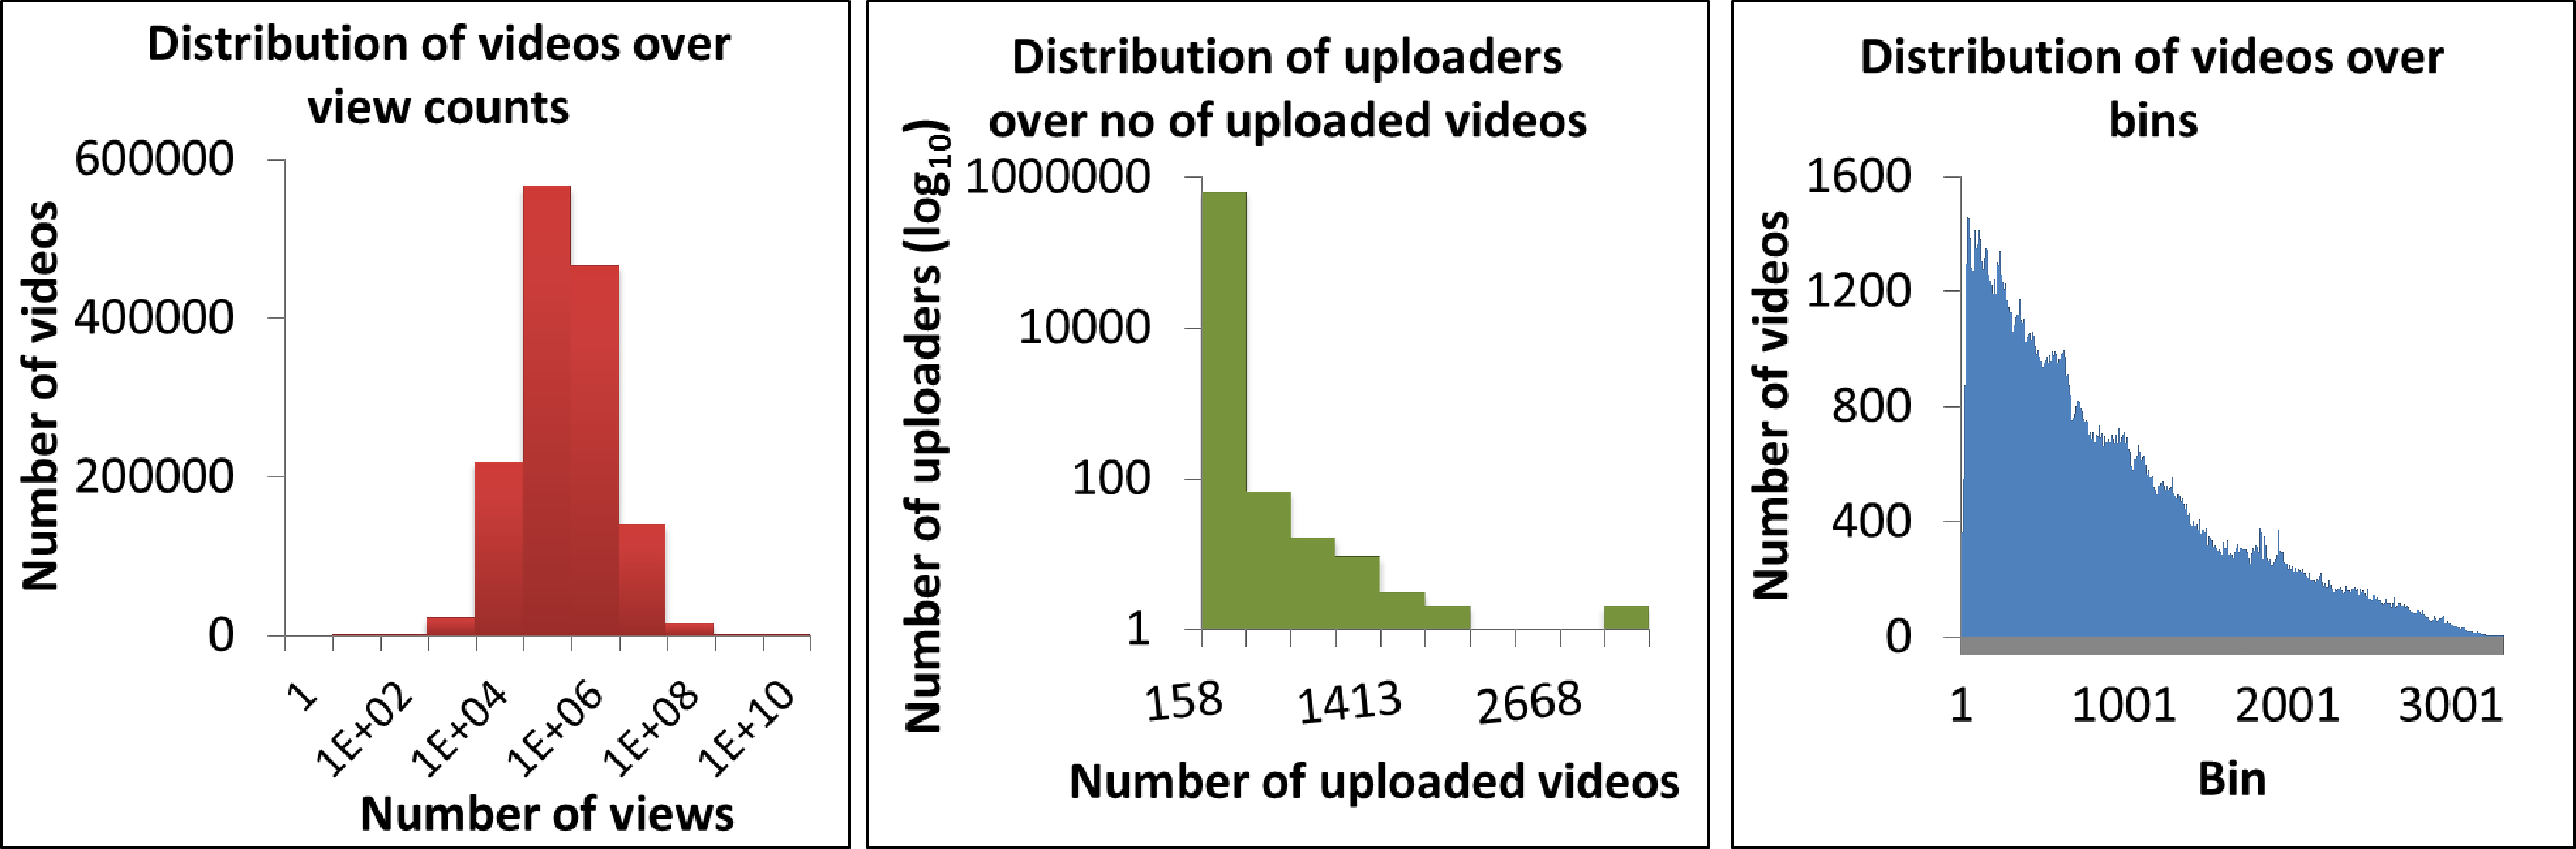
\includegraphics[width=1.0\textwidth,clip]{distributions.pdf}
			\end{center}
			\caption{Red-colored histogram: Distribution of videos over view counts. Blue-colored histogram: Distribution of uploaders over number of uploaded videos. Green-colored histogram: Distribution of number of videos in each bin.}
			\label{fig:histograms}
		\end{figure}
	
		As the statistics show, we have a large magnitude in ranges of number of view, likes and dislikes. This motivates us to do some preprocessing on data, such as feature normalization or data standardization, to ensure the numerical stability and good speed of convergence on the learning algorithm for logistic regression. We discuss more on this step in the Section \ref{sec:orderofmagnitude}.
						
	\subsubsection{Feature extraction}
		In this section we discuss the feature engineering process in the project. First, we build a dictionary mapping the uploader to the number of videos they have uploaded and the total number of views there videos have. We also take care to prevent "cheating":  In order to ensure that our predictor has only such information as would be available before the video's publishing is ever used, we temporarily reduce these number of video-views and the total number of video uploads for the uploader according to the publish date of the video under current consideration.

		We considered many features, which ultimately include:
		\begin{itemize}
			\item
			Features extracted via a bag-of-words model on the title, using TF-IDF.
			\item
			The number of videos uploaded by the uploader prior to the current video's upload date.  Because of our desire for caution against "cheating", we count only those videos that we have crawled.
			\item
			The total number of views for the uploader due to videos released prior to the current video's upload date.  Again, we count only those videos that we have crawled.  This date-conscious counting is particularly important because there are many cases where there is only one video crawled for a given uploader, meaning that this feature would become a nearly perfect predictor.
			\item
			The number of subscribers for the uploader.  We lack sufficient data to know how subscribers changed over time, so we simply had to keep this constant.
			\item
			The runtime of the video, in seconds.
			\item
			The age of the video at the time of crawling, in days.
			\item
			The number of likes/dislikes.  Since these are expected to scale with the number of views, we forbade ourselves from using the number directly, but we did allow certain combinations, such as the log of the like-vs-dislike ratio.
			\item
			Various combinations of the above features (for example, the log of some other feature, or the ratio between two features).
		\end{itemize}
	
\subsection{Evaluation Metrics}
	Normally, a rank correlation \footnote{http://en.wikipedia.org/wiki/Rank\_correlation} is a common metric in ranking problems. Since our problem is re-formulated as a classification and regression problems, we evaluate our methods using corresponding metrics such as Root Mean Square Error (RMSE) for Regression and $F_1$-score and Accuracy for Classification.
	
	\subsubsection{Classification}
	The error matrix (or confusion matrix) is a common way to measure performance of any arbitrary classifiers. Several metrics derived from this matrix are Accuracy, Precision-Recall, $F_1$-score or Receiver Operator Characteristics (ROC). In our work we employ two of them: Accuracy and $F_1$-score \footnote{http://en.wikipedia.org/wiki/F1\_score}.
	
	The accuracy can be equivalently stated as a 0-1 loss function over total number of pairs in testing set.
	\begin{equation}
		0/1_{loss} = \sum_{(u, v)_{test}} \frac{1}{|(u,v)_{test}|} \textbf{1}[\hat{Y}_{uv} - Y_{uv} == 0]
	\end{equation}
	
	\subsubsection{Regression}
	To Joseph: Can you put your least square formula here ? The first few paragraphs in section 4.3.2 can be put here. And show the equations as well.
